\section{Implementation choices}
\label{sec:03-implementation}
Describe the choices with links to the previous section.
Insert pseudocode of the implementation.

As stated in \cref{sec:motion-models}, we decided to use an indirect method with affine model for motion estimation as in \cite{Bergen92}.
Also, we decided to obtain a robust estimation by using a strategy similar to \cite{Dufeaux2000}, where they adopt a hierarchical approach to obtain a robust estimation using coarse resolution to guide the search for the best parameters at a finer resolution.

In the following sections, we will explain the implementation choices in detail and present the pseudocode of the algorithm. A schematic representation of the algorithm is presented in \cref{fig:gme-schema}.

\begin{figure}
    \centering
    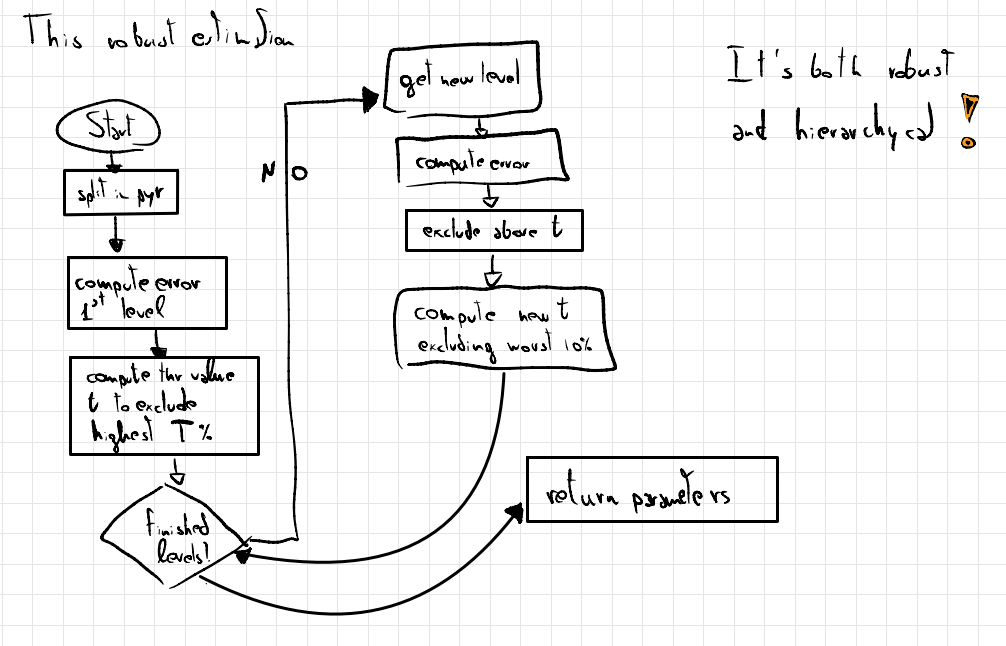
\includegraphics[width=.95\linewidth]{../assets/images/gme-schema.png}
    \caption{Schema of the flow of implementation of the global motion estimation pipeline.}
    \label{fig:gme-schema}
\end{figure}

\subsection{Block Matching Motion Estimation}
The first piece of the architecture is the algorithm to compute the motion field to be used as ground truth.
In our case, we decided to implement a block matching motion estimation (BMME), because computing the motion field on blocks, rather than single pixels, can be much less computationally expensive.

The main idea of BMME is to divide the frame in blocks, and search for each block in the previous frame the corresponding block in the next frame.
This gives us the displacement of the block between the two frames, which is treated as the motion vector of the block.
This is the basic principle of BMME, from which derived a number of implementations that present differences mainly in two aspects:
\begin{enumerate}
    \item the size and shape of the block;
    \item the path that the searching procedure follows.
\end{enumerate}

During the project we implemented a number of these techniques:
\begin{itemize}
    \item exhaustive search;
    \item two-dimensional logarithmic search;
    \item three-step search, from \cite{Li94};
    \item diamond search, from \cite{Zhu2000};
\end{itemize}

In the final implementation, the block matching method used is the one presented in \cite{Zhu2000}, known as diamond search (DS),  with a mean square error measure to compute (dis-)similarity between blocks.
Nonetheless, all the other methods are still present and by slightly changing the code they can be tested as well.

Here we briefly discuss the algorithm that we choose to implement and propose a small example for clarification.
The DS algorithm defines a peculiar diamond-shaped search pattern, which defines which positions will be used as target points where to center the block in the next frame to see if it corresponds to the block in the previous frame.

The procedure is the following:
\begin{enumerate}
    \item the search starts with a large diamond, meaning that we check the blocks centered in each one of the 9 positions defined by the large diamond, if the best match is the central position then we pass to the second step, otherwise we move to the best match position and re-use the large diamond;
    \item in the second step we use a smaller diamond shape and look again for the best matching position among the 5 possible defined by the small diamond, then return the best match position.
\end{enumerate}

\begin{figure}
    \centering
    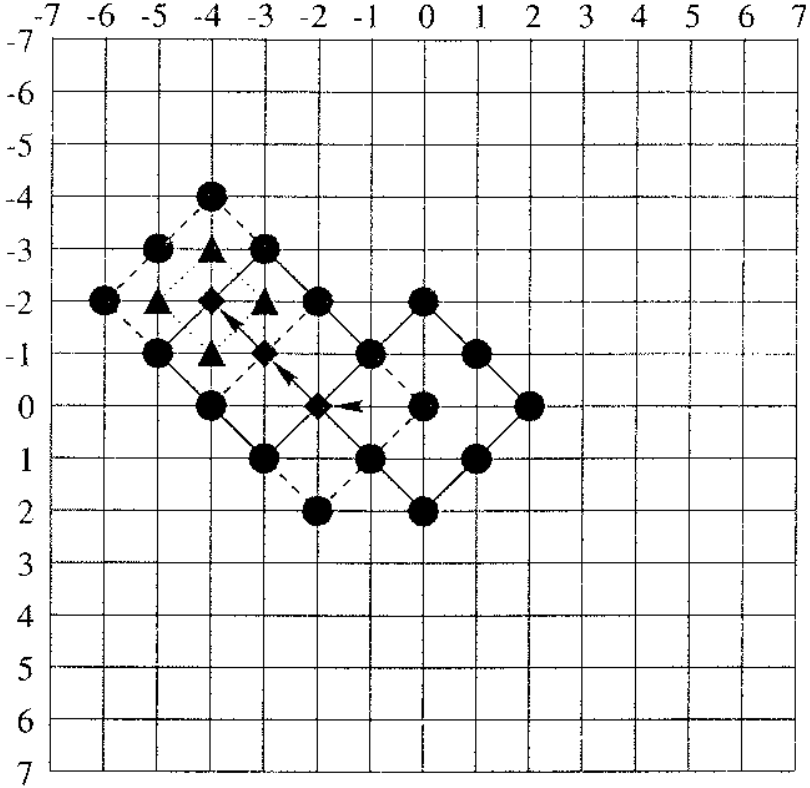
\includegraphics[width=.95\linewidth]{../assets/images/ds-exe.png}
    \caption{Example of run of diamond search algorithm for block matching motion estimation.}
    \label{fig:diamond-search-example}
\end{figure}

In \cref{fig:diamond-search-example} we can see an example of run. We can spot the three large-shape diamonds (the contour position are marked with circles) and the small shaped diamond (contour positions marked with triangles).
In this example the block matching algorithm started from $\{0,0\}$, then moved with the large diamond to $\{-2,0\}$, because this was the position that minimized the error between the block in the previous and the next frame. Then again with the large diamond the algorithm reached $\{-3,-1\}$ first, and $\{-4,-2\}$ after. Here the best matching position for the large diamond shape was $\{-4,-2\}$, therefore the algorithm stopped using the large diamond and started with the small diamond. Finally, the small diamond returned once again as best match position $\{-4,-2\}$, which was then returned as final matching position for the block in the previous frame.

\subsection{Affine Model Parameter Estimation}
In \cref{sec:motion-models}, we presented the affine motion model, which is the one we decided to use in our implementation.

To get the motion vector of a certain position $\{x,y\}$ in the previous frame, we can solve the following matrix formulation of the model:
\begin{equation}
    d(p, a) = A(p)\;a
\end{equation}
where $d(p, a)$ is the displacement for the position $p$, given the parameter vector $a$; $A(p)$ is an intermediate matrix that is computed as 
\begin{equation*}
    A = \begin{bmatrix}
        1 & x & y & 0 & 0 & 0 \\
        0 & 0 & 0 & 1 & x & y
    \end{bmatrix}
\end{equation*}

\red{copy here formulas page 188}




\subsection{Hierarchical Robust Estimation}